\documentclass[conference]{IEEEtran}
\usepackage{url}
\usepackage{graphicx}
\usepackage{subfigure}

\newcommand{\todo}[1]{\textbf{TODO}\footnote{\textbf{TODO:} #1}}

\begin{document}

\title{The GHTorrent dataset and tool suite}

\author{\IEEEauthorblockN{Georgios Gousios} 
\IEEEauthorblockA{
Software Engineering Research Group\\
Delft University of Technology\\
Delft, The Netherlands\\
Email: g.gousios@tudelft.nl}
}

\maketitle

\begin{abstract}
Foo
\end{abstract}

\begin{IEEEkeywords}
Git, pull request, collaborative development
\end{IEEEkeywords}

\section{Introduction}
During the recent years, Github has been taking 

\begin{figure}
  \begin{center}
    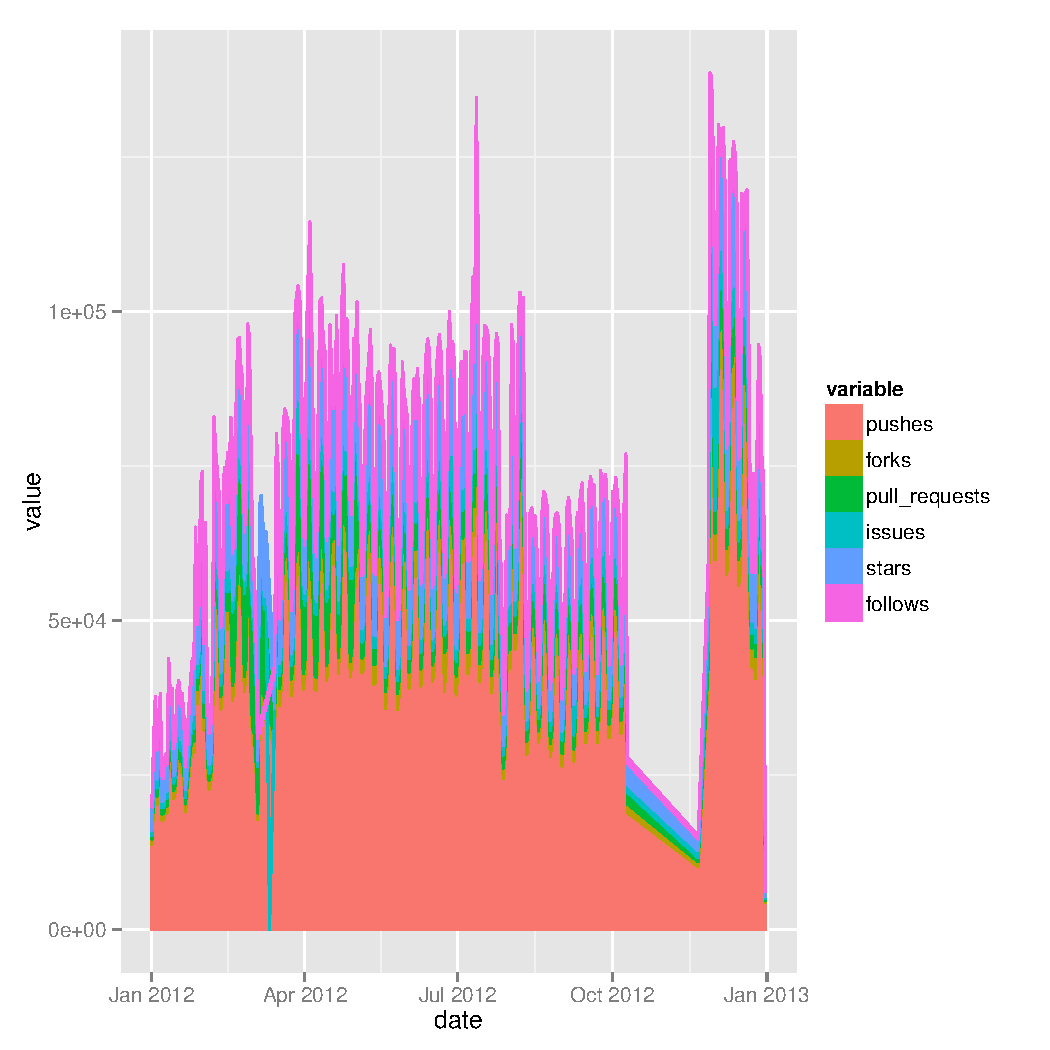
\includegraphics[scale=0.3]{github-growth}
  \end{center}
  \caption{Github's growth in terms of emitted events}
  \label{fig:growth}
\end{figure}

The proposed data collection scheme was first presented in~\cite{GS12}.
Since this work, the data collection process has been fully
implemented, the data schema has been stabilized and a new service
to collaboratively collect and query the data has been implemented.
In this paper, we focus on the newest developments and present
characteristics of the dataset to 

\section{Data schema}

\begin{table*}
  
  \begin{center}
    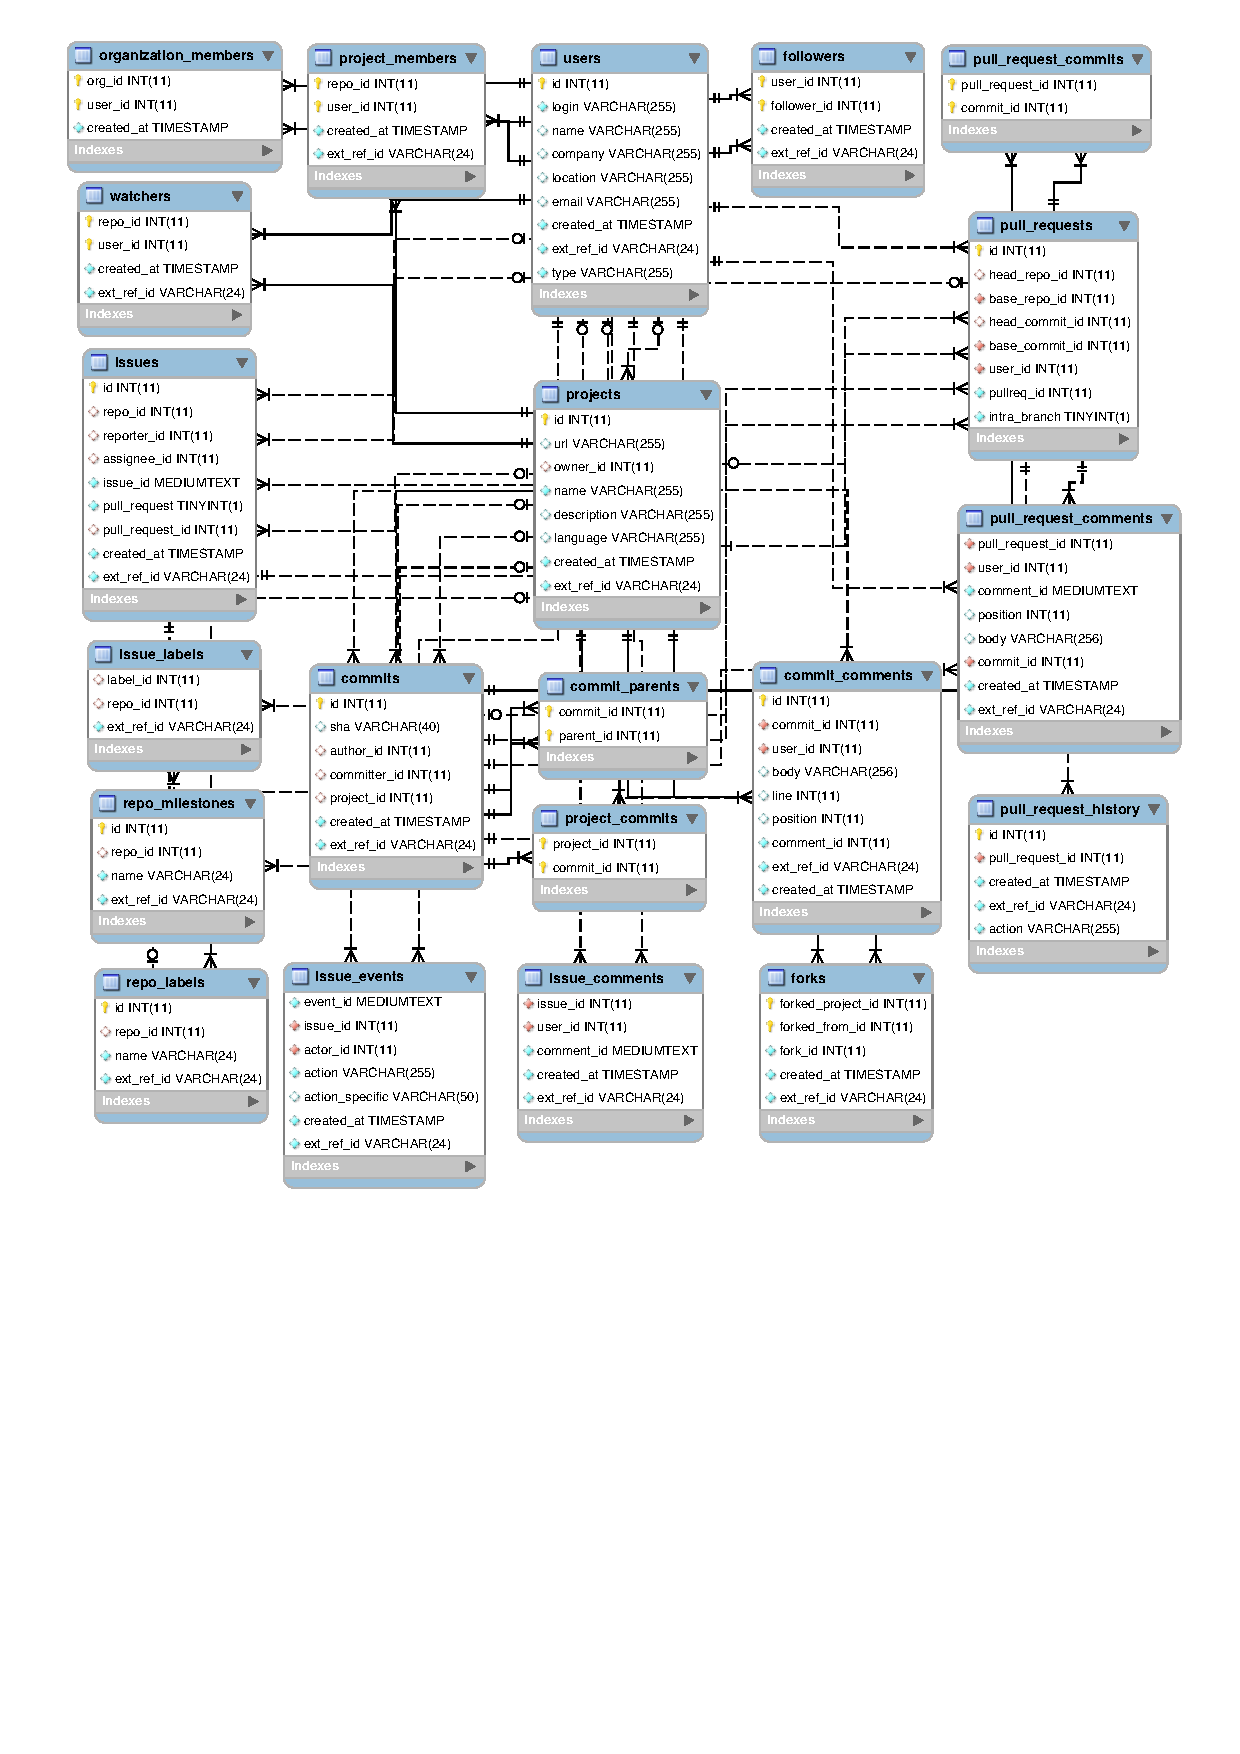
\includegraphics[scale=0.74]{ghtorrent-schema.pdf}
  \end{center}
  \centering
  \begin{tabular}{lp{25em}p{8em}l}
      \hline
      \bf{Entity} & \bf{Description} & \bf{Raw data entity} & \bf{Num Items} \\
      \hline
      \sf{projects} & Project repositories & \tt{repos} & 652.665\\
      
      \sf{users} & Github users. & \tt{users} & 589.101\\
      
      \sf{project\_members} & Users with commit access to the referenced
      \sf {project}. & \tt{repo\_collabs} & 773.307\\
      
      \sf{organization\_members} & List members of an organization ``\sf{user}'' & \tt{org\_members} & 34.924\\

      \sf{forks} & Forks of a \sf{project} & \tt{forks} & 1.106.469\\

      \sf{commits} & A list of all commits on Github. The \sf{project\_id} field
      refers to the first \sf{project} this commit has been done to &
      \tt{commits} & 23.886.460\\
      
      \sf{project\_commits} & List of all \sf{commits} to a \sf{project}.& --- &
      ---\\

      \sf{commit\_parents} & Commits that are parents to a \sf{commit}.& --- & ---\\
      
      \sf{commit\_comments} & Code review comments for a \sf{commit}.& \tt{commit\_comments} & 82.133 \\
      
      \sf{watchers} & \sf{user}s that have starred (was watched) a \sf{project} & \tt{watchers} & 6.153.510\\

      \sf{followers} & \sf{user}s that are following another \sf{user}
      \sf{project}& \tt{followers} & 1.447.713\\

      \sf{issues} & Issues that have been recorded for a \sf{project}.&
      \tt{issues} & 1.765.821 \\
      
      \sf{issue\_events} & Chronologically sortable list of events on an
      \sf{issue}. & \tt{issue\_events} & 3.484.944 \\
      
      \sf{issue\_comments} & Discussion comments on an \sf{issue} &
      \tt{issue\_comments} & 2.247.567 \\
      
      \sf{pull\_requests} & List of pull requests for \sf{base\_repo}. Requests
      originate at head \sf{head\_repo}/\sf{commit} and are created by
      \sf{user\_id} & \tt{pull\_requests} & 929.037 \\ 
 
      \sf{pull\_request\_comments} & Discussion comments on a \sf{pull\_request}
      &  & 288.850\\

      \sf{pull\_request\_history} & Chronologically sortable list of events on
      on a \sf{pull\_request} & --- & ---\\

      \hline
    
  \end{tabular}
  \caption{Schema entities, their description, the corresponding raw data
  entities and the number of raw data items (Jan 2013).}
  \label{tab:entities}
\end{table*}

\section{Data Collection}

The 

To cope with the volume of data and the fact that Github imposed a request limit
of 5.000 requests per hour,

The data collection was designed from the beginning
as a decentralized process. Decentralization is mediated using the worker queue
model; a message producer sends messages to the appropriate queue and several
workers process messages, perform the requests and store the results in a common
database. There are two types of messages whose processing can be distributed:

\begin{itemize}

  \item Events: Those correspond to entries in the Github event stream. The
    \texttt{retrieve-data} client uses them to update

  \item Repository names (format \texttt{owner/repo}): The \texttt{retrieve-repo} tool
    uses the information to retrieve all available information for a single
    project repository. As getting the commits for a repository requires an
    excessive amount of {\sc api} calls to be performed, an extra tool, 
    \texttt{get-more-commits}, has been written to retrieve the full list of commits
    on request. 

\end{itemize}

Decentralization enables collaborating researchers to contribute to the data
collection effort, by simply installing the GHTorrent command line client and
configuring it to connect to the central repository databases. 

\section{Research Opportunities}



\section{Challenges and Limitations}

From a repository mining prespecive, the GHTorrent dataset has the following
limitations. 

\begin{itemize}

  \item \emph{Data is additive:} Github is a dynamic site where developers, 
    projects and wikis are created and deleted constanly. Despite the fact
    that the Github event stream reports additions of entities, it does
    not report deletions. This means that the information in the GHTorrent 
    database cannot be updated when a user or a repository has been marked
    as deleted. This can have several consequences 

  \item \emph{Important entities are not timestamped:} Github does not report
    timestamps for the watchers/stars and followers entities. This means that it
    is not possible to query the followers for a user or the watchers for a
    repository at a specific timestamp. As a workaround, GHTorrent uses the
    timestamp of the event that is generated when a follow/watch action is
    performed, but this is only limited to the events that took place since
    the GHTorrent project started its data collection.

  \item \emph{Issues and pull requests} Issues and pull requests are dual on
    Github; for each opened pull request, an issue is opened automatically, if
    the project has enabled the issue tracker. Commits can also be attached to
    issues to convert them to pull requests (albeit with external tools). This
    duality has the following implications: 

    \begin{itemize}

      \item Discussion comments for a pull request need to be retrieved from
        multiple sources, namely from {\sf commit\_comments} for code reviews,
        from {\sf issue\_comments} if the pull request is also an issue and 
        from {\sf pull\_request\_comments} if the issue tracker is not enabled
        for a project.

      \item There are two different status entities that need to be queried to
        get the succession of events on a pull request.

    \end{itemize}

  \item \emph{Commit users:} Git allows users to setup  

  \item \emph{Pull requests merged outside Github:} Despite the fact that Github
    automates the generation and submission of patches among repositories
    through pull requests, those need not be merged through the Github
    interface. Indeed, several projects choose to track the discussion on pull
    requests using Github's facilities while doing the actual merge using
    {\sf git}. A researcher can observe this behaviour because an usually big
    number of pull requests are closed without being reported as merged.
    Unfortunatelly, there is no precise way to tell whether those pull requests
    have been indeed merged, except by resolving to commit log mining
    heuristics.

  \item \emph{Trivial projects:} The majority of projects in Github are forks of
    another project (\todo{Run query}). Of the remaining projects, several are
    trivial, containing only a few commits, while many do not contain source
    code (for example, Github pages repositories). To obtain a list of projects
    worth investigating, the researcher should filter the remaining projects
    for specific properties (for example, popularity, programming language etc).

  \item \emph{Some data may be missing:} 
    Mulfunctions in the mirroring system (software or network) can result in 
    some parts of the data that are missing. In principle, apart from
    events, all missing data in GHTorrent can be restored (by replaying the
    event log or using the \texttt{ght-retrieve-repo} script) provided that the
    original data have not been deleted from Github. In the case of missing
    events, the current Github {\sc api} does not permit retrieving more than
    the 300 newest per repository. On busy projects, this is less than
    a day's worth of event log. Known periods of missing events 

  \item \emph{Issue tracking is open ended:} Repository mining for bug tracking
    repositories is greatly enhanced, if records are concistent accross
    projects. This is why most studies have been carried on Bugzilla data, which
    offers a good default set of properties per bug and little opportunities to
    customize the bug report further. On the other hand, Github's bug tracker
    only requires a textual description to open a bug. Bug property annotations
    (e.g. affected versions, severity levels) are delegated to project specific
    labels. This means that in principle characteristics of bugs cannot be
    examined uniformly across projects.

\end{itemize}


\section{Conclusions}

\section*{Acknowledgements}
This work is funded by Marie Curie {\sc ief} 298930 -- {\sc sefunc}.

\bibliographystyle{ieeetr}
\bibliography{ghtorrent-data}

\end{document}
